\section{Transformationspfade in der Energiewirtschaft}

\textbf{Energiepolitische Herausforderungen:} Weltbevölkerung steigt $\rightarrow$ Primärenergieverbrauch steigt $\rightarrow$ Steigende CO\textsubscript{2} Emissionen weltweit

\textbf{Energiewirtschaftliche Viereck:} Forderung nach gesicherter, bezahlbarer, umweltfreundlicher, akzeptierter Energieversorgung

\textbf{CO\textsubscript{2}-Emissionen in Deutschland}: Die meisten CO\textsubscript{2}-Emissionen im Energiesektor durch Stein- und Braunkohle $\rightarrow$ Tendenz sinkend

\textbf{Energiepolitische Ziele in Deutschland:}
\begin{itemize}
	\item Treibhausgasemissionen sollen bis 2030 um 65\% sinken (im Vergleich zu 1990)
	\item Ausbau erneuerbarer Energien
	\item Erhöhung des Anteils erneuerbarer Energien am Bruttostromverbrauch bis 2030 auf 80\%
	\item Reduzierung des Primärenergieverbrauchs bis 2050 um 50\% (im Vergleich zu 2008)
\end{itemize}
\bigskip
\textbf{Herausforderungen für deutsches Stromsystem:}
\begin{itemize}
	\item Paradigmenwechsel durch die Integration von erneuerbarer Energie
	\item Veränderte Angebots- und Nachfragestruktur $\rightarrow$ Zentral zu dezentral $\rightarrow$ Verlagerung von Großkraftwerken hin zu kleinen dezentralen Erzeugungseinheiten und neue Konsumenten wie Elektrofahrzeuge
\end{itemize}
\bigskip
\textbf{Auswirkung von erneuerbarer Energie auf das Merit-Order Modell:}
\begin{center}
	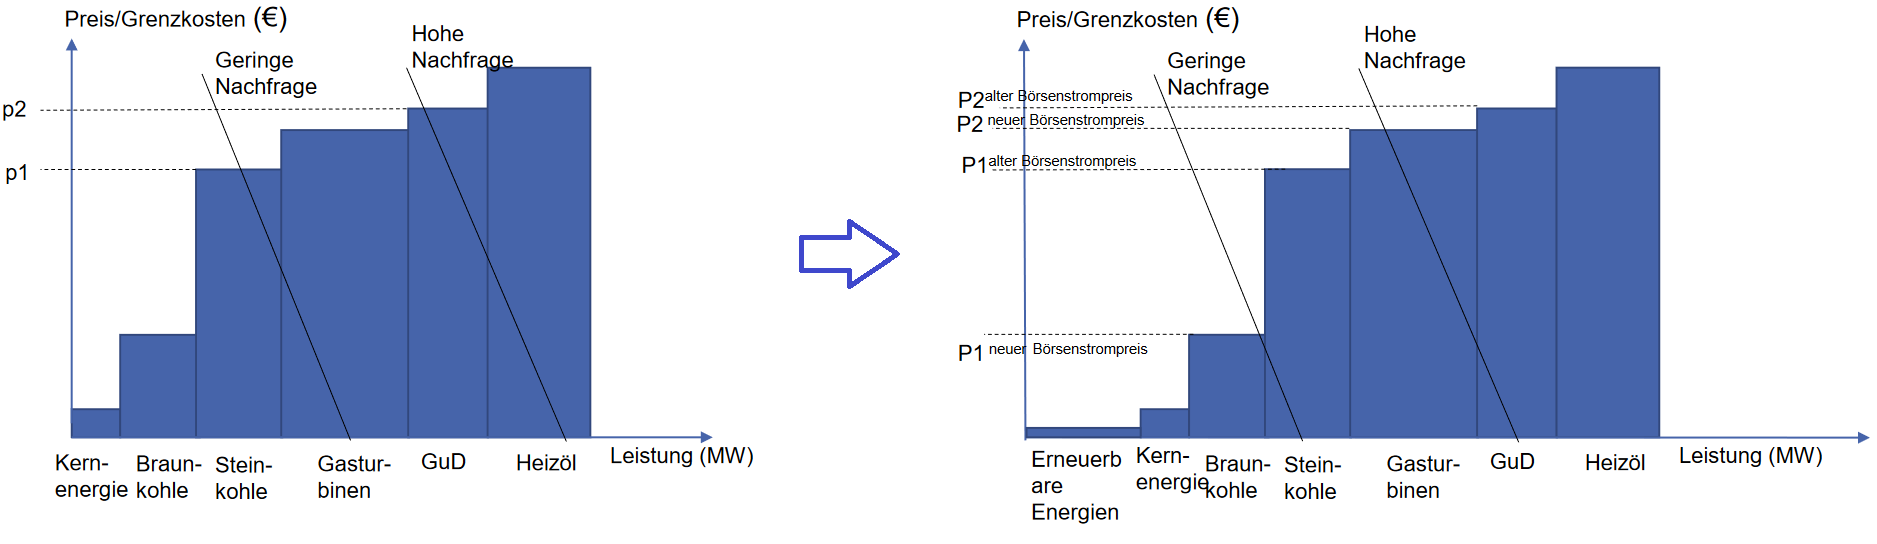
\includegraphics[width=\textwidth]{images/merit-order.png}
\end{center}
\begin{itemize}
	\item \textbf{Merit-Order}: Kraftwerkseinsatzreihenfolge basierend auf den Grenzkosten der Elektrizitätserzeugung
	\item Kraftwerksreihenfolge wird durch erneuerbare Energien verschoben $\rightarrow$ Strompreis sinkt
\end{itemize}
\pagebreak
\textbf{Strompreis:}
\begin{center}
	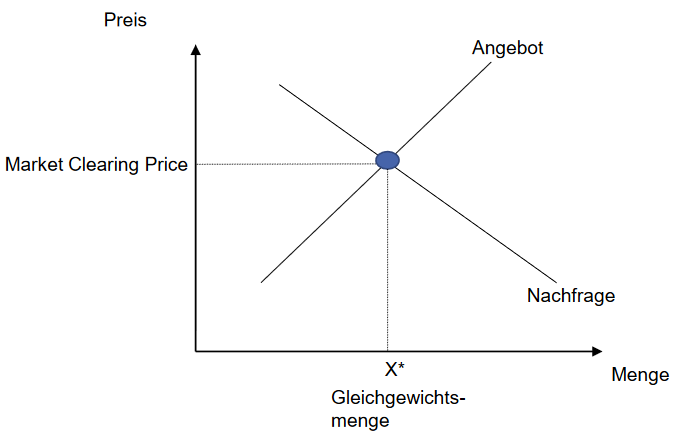
\includegraphics[width=0.6\textwidth]{images/strompreis.png}
\end{center}
\begin{itemize}
	\item Börsenpreis entspricht dem Schnittpunkt von Angebot und Nachfrage
	\item \textbf{Market Clearing Price} entspricht den Grenzkosten des letzten Kraftwerks, dass zur Deckung der Stromnachfrage benötigt wird
\end{itemize}
\bigskip
\textbf{Klimaschutzziele (KSG):}
\begin{itemize}
	\item 2030: 15 Mio. Elektrofahrzeuge
	\item 2030: 85 Mio. \si{\tonne} CO\textsubscript{2} (2021: 148 Mio. \si{\tonne} CO\textsubscript{2})
	\item 2045: CO\textsubscript{2}-frei
\end{itemize}